
\chapter{Appendix B: Statistical Significance Tests}

\renewcommand{\thechapter}{B}

\section{Test Setup}
\label{sec:significance_setup}

The paired Wilcoxon signed-rank test, paired $t$-test, Shapiro-Wilk
normality test, and Cohen's $d$ are defined in
Section~\ref{sec:significance_bg}. This appendix records only the
choices specific to the evaluation pipeline.

All tests are two-sided with $\alpha = 0.05$. The Wilcoxon $p$-value is
reported as the primary statistic, since per-query retrieval metrics
are heavily non-normal. Win, tie, and loss counts are computed by
direct per-query comparison of the two score vectors.

In addition to the per-subset tests, a pooled \emph{mean} test is
computed by concatenating per-query scores from all 13 NanoBEIR subsets
into a single paired sample, preserving pairing within each subset.
This pooled test assesses whether one model is significantly better
than the other across the full evaluation set, rather than on any
individual subset.

\section{BGE: Pre-trained vs Fine-tuned at MRR@10}
\label{sec:significance_bge_finetune}

Per-query MRR@10 is recorded for both pre-trained BGE-base-en-v1.5 and
its MNRL fine-tuned counterpart on the 13 NanoBEIR subsets. Pooling
across subsets while preserving within-subset pairing yields the test
sample summarised in Table~\ref{tab:sig_bge_finetune}.

\begin{table}[h]
    \centering
    \caption[BGE pre-trained vs fine-tuned: significance summary]%
    {Paired significance summary for pre-trained vs MNRL fine-tuned
    BGE-base-en-v1.5 on per-query MRR@10, pooled across the 13
    NanoBEIR subsets. Positive Cohen's $d$ favours the pre-trained
    model.}
    \label{tab:sig_bge_finetune}
    \begin{tabular}{l r p{0.55\textwidth}}
        \toprule
        \textbf{Parameter} & \textbf{Value} & \textbf{Description} \\
        \midrule
        $n$               & 649        & Paired per-query observations pooled across the 13 NanoBEIR subsets. \\
        Wins              & 82         & Queries where pre-trained MRR@10 $>$ fine-tuned. \\
        Ties              & 490        & Queries where both models return identical MRR@10. \\
        Losses            & 77         & Queries where fine-tuned MRR@10 $>$ pre-trained. \\
        Cohen's $d$       & $+0.035$   & Effect size on the difference vector; well below the $|d| \approx 0.2$ small-effect threshold. \\
        Shapiro--Wilk $p$ & $<10^{-3}$ & Rejects normality of the paired differences; motivates the Wilcoxon test in preference to the paired $t$-test. \\
        Wilcoxon $p$      & $0.486$    & Two-sided paired signed-rank test; fails to reject $H_0$ of zero median difference at $\alpha = 0.05$. \\
        \bottomrule
    \end{tabular}
\end{table}

The 75\,\% tie rate (490 of 649 queries) shows that for most queries
the two models return identical top-10 orderings; the remaining
differences are small and balanced in direction, leaving no
statistically detectable shift in retrieval quality.

\begin{figure}[h]
    \centering
    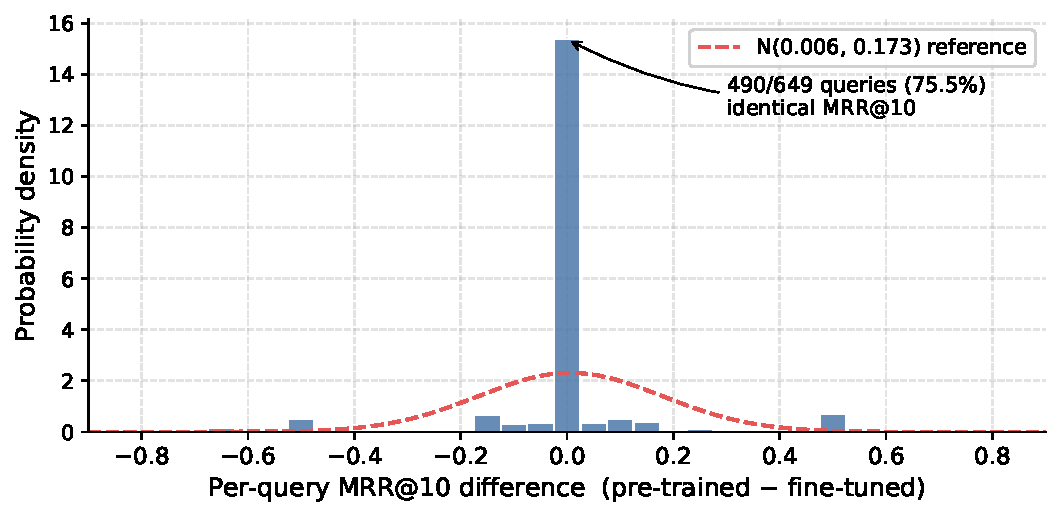
\includegraphics[width=0.75\textwidth]{Figures/fig_sig_bge_finetune_diffhist.pdf}
    \caption[Distribution of per-query MRR@10 differences: pre-trained
    vs fine-tuned BGE]{Distribution of per-query MRR@10 differences
    (pre-trained $-$ fine-tuned) for BGE-base-en-v1.5, pooled across
    the 13 NanoBEIR subsets ($n = 649$). The red dashed curve is the
    maximum-likelihood normal fit. The distribution is sharply
    concentrated at zero and the non-zero mass is roughly symmetric,
    making the normal fit a poor model and motivating the
    non-parametric Wilcoxon test reported in
    Table~\ref{tab:sig_bge_finetune}.}
    \label{fig:sig_bge_diffhist}
\end{figure}

\section{Binarisation-Aware Training Exceeds Float32 on RoBERTa}
\label{sec:significance_bat_roberta}

Per-query MRR@10 is recorded for the RoBERTa float32 fine-tune and
for each of its two binarisation-aware variants (BAT-STE and
BAT-atanh) on the 13 NanoBEIR subsets. Pooling across subsets while
preserving within-subset pairing yields the test sample summarised
in Table~\ref{tab:sig_bat_roberta}. Positive Cohen's $d$ favours the
binarised variant.

\begin{table}[h]
    \centering
    \caption[BAT vs float32 on RoBERTa: significance summary]%
    {Paired significance summary for BAT-STE and BAT-atanh against
    the RoBERTa float32 fine-tune on per-query MRR@10, pooled across
    the 13 NanoBEIR subsets.}
    \label{tab:sig_bat_roberta}
    \begin{tabular}{l r r p{0.45\textwidth}}
        \toprule
        \textbf{Parameter} & \textbf{BAT-STE} & \textbf{BAT-atanh} & \textbf{Description} \\
        \midrule
        $n$               & 649        & 649        & Paired per-query observations pooled across the 13 NanoBEIR subsets. \\
        Wins              & 155        & 167        & Queries where the binarised variant scores higher. \\
        Ties              & 361        & 370        & Queries where both models return identical MRR@10. \\
        Losses            & 133        & 112        & Queries where the float32 fine-tune scores higher. \\
        Cohen's $d$       & $+0.117$   & $+0.207$   & Effect size on the difference vector; both favour the binarised variant. \\
        Shapiro--Wilk $p$ & $<10^{-3}$ & $<10^{-3}$ & Rejects normality of the paired differences; motivates the Wilcoxon test in preference to the paired $t$-test. \\
        Wilcoxon $p$      & $0.005$    & $<10^{-3}$ & Two-sided paired signed-rank test; rejects $H_0$ of zero median difference at $\alpha = 0.05$ in both cases. \\
        \bottomrule
    \end{tabular}
\end{table}

Both tests reject the null of zero median difference at
$\alpha = 0.05$, and both effect sizes point the same way: the
binarised variant scores higher than the float32 fine-tune on
average per query. The gain is therefore real, not a sampling
artefact, and BAT-atanh shows the larger effect of the two.
